\section{Durchführung}
\label{sec:Durchführung}

\subsection{Versuchsaufbau}
\label{subsec:Versuchsaufbau}

Der Versuch wird nach \autoref{fig:aufbau} aufgebaut. 
\begin{figure}[H]
    \centering
    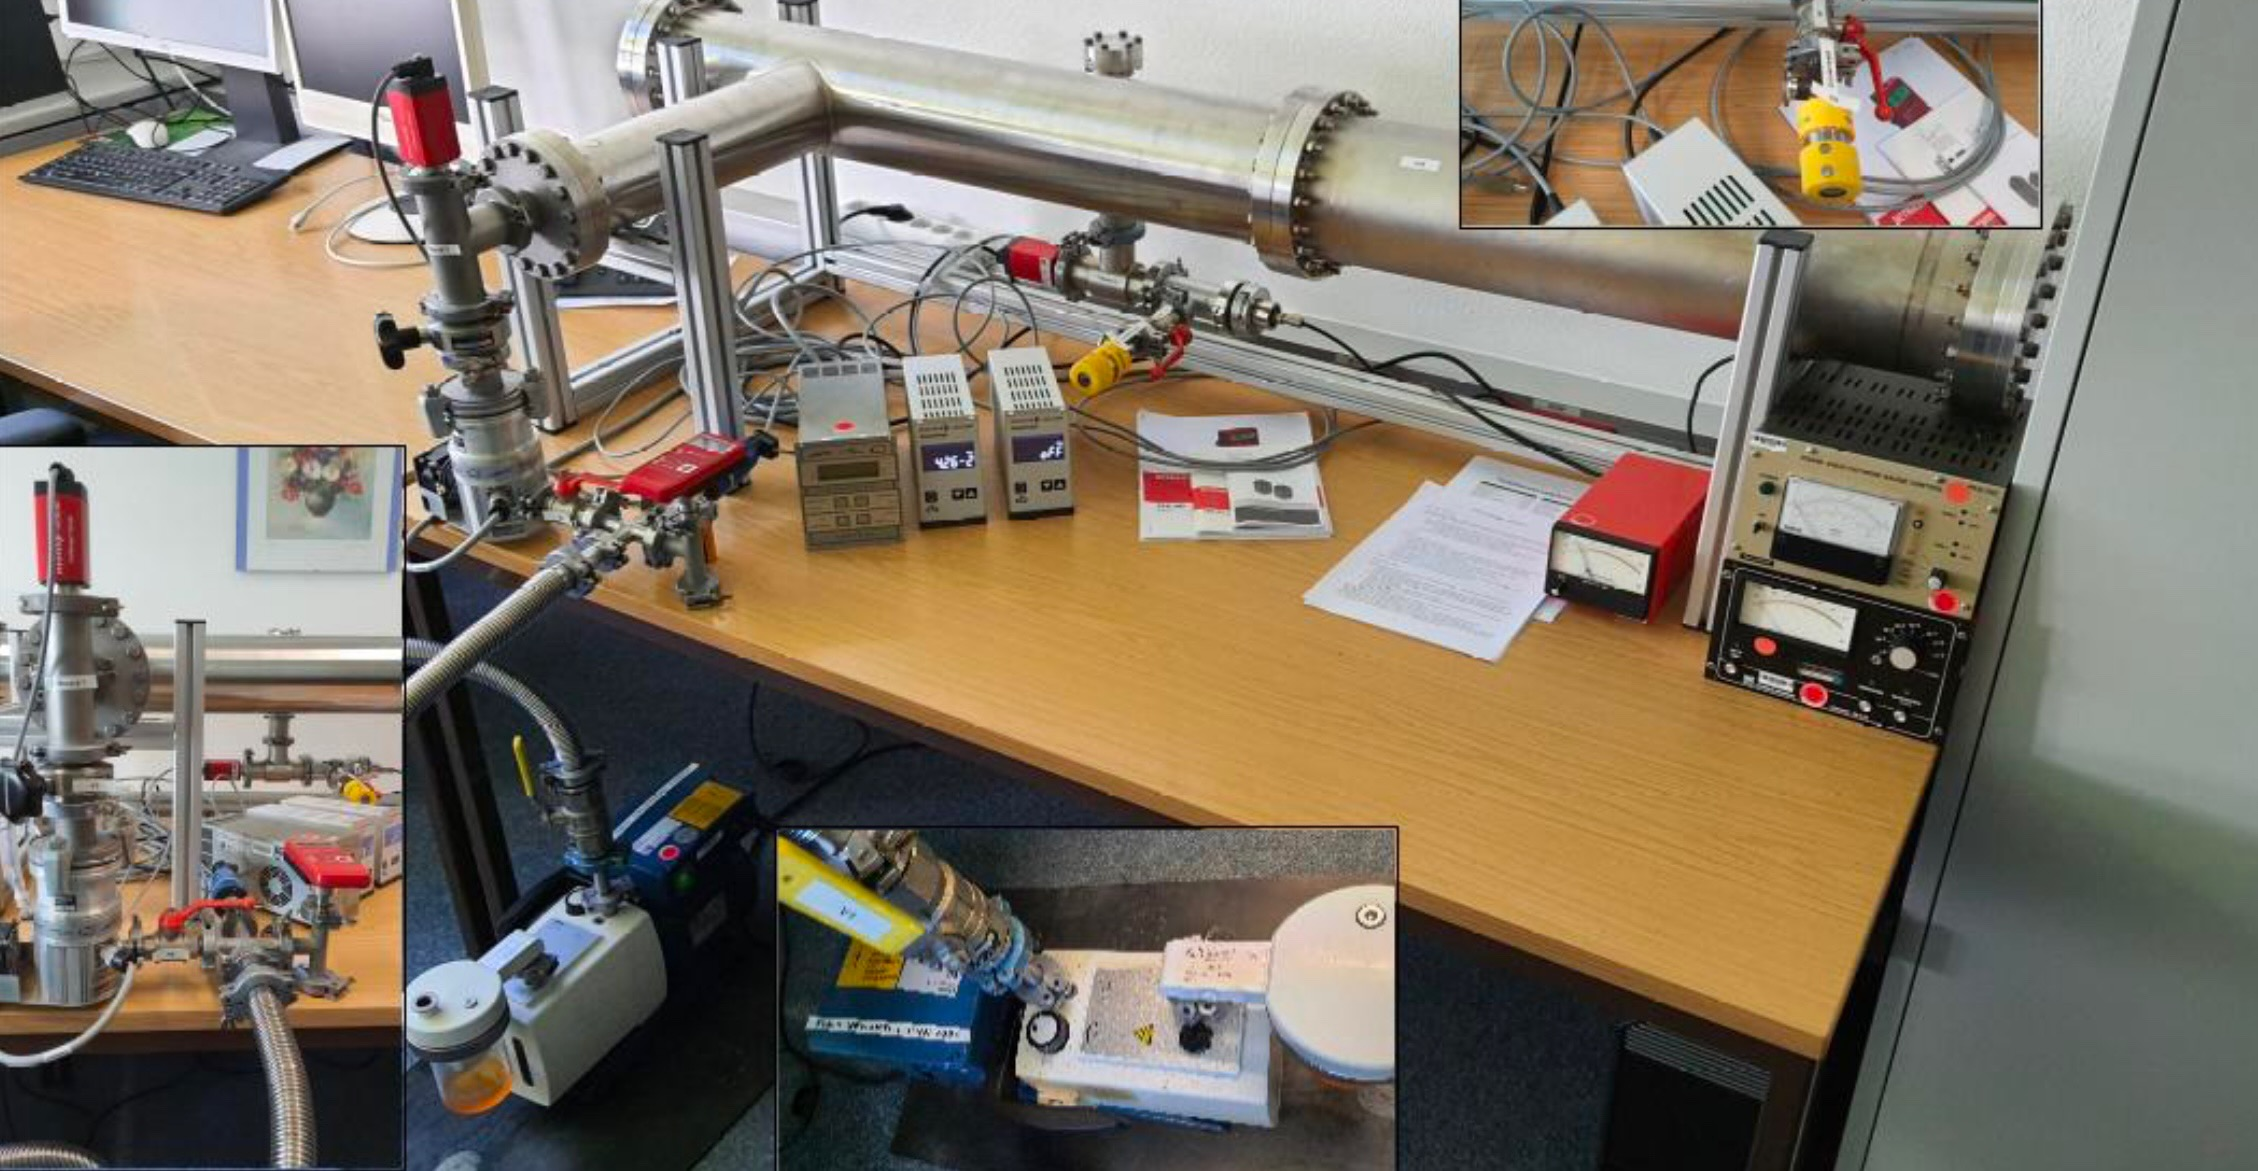
\includegraphics[width=\textwidth]{data/Versuchsaufbau.jpeg}
    \caption{Aufbau des Versuches \cite{Anleitung70}.}
    \label{fig:aufbau}
\end{figure}

\noindent
Im Versuch wurde eine Drehschieberpumpe der Firma ILMVAC Typ 300883/AKD16 mit einem Saugvermögen von $\SIrange{4,6}{5,5}{\cubic\meter\per\hour}$ und einem Enddruck von $\SI{2 e-3}{\milli\bar}$ verwendet. \newline
Die Turbomolekularpumpe SST81 von der Firma ILMVAC wird bei einer Frequenz von $\SI{1350}{\hertz}$ betrieben. Die Herstellerangabe für das Saugvermögen beträgt $\SI{77}{\litre}$.
Als Messgeräte wurden die folgenden beiden Geräte verwendet:
\begin{enumerate}
    \item PKR 360, Pfeiffer Vacuum, kombinierter Pirani/Kaltkathode-Sensor (2 x rote Messgeräte verbaut am Rezipienten) ausgelesen mit 2 x Anzeigegeräte TPG 361, Pfeiffer Vacuum („SingleGauge“):
    Messbereich: $\SIrange{10 e-9}{1000}{\hecto\pascal}$; Messgenauigkeit ($N_2$): $\SIrange{10 e-8}{100}{\hecto\pascal}$ bei $30 \%$ des Messwertes und
    $\SIrange{100}{1000}{\hecto\pascal}$ bei $50 \%$ des Messwertes 
    \item TPG202, Pfeiffer Vacuum, kombinierter Piezo/Pirani-Sensor:
    Messbereich: $\SIrange{1200}{5 e-4}{\hecto\pascal}$; Messgenauigkeit: $\SIrange{1200}{10}{\hecto\pascal}$ mit $0,3 \%$ vom Vollausschlag, $\SIrange{10}{2 e-3}{\hecto\pascal}$ mit $10\%$ vom Vollausschlag.
    Bei $\leq \SI{2 e-3}{\hecto\pascal}$: < Faktor 2 vom Messwert.
\end{enumerate}

\noindent
Die Volumina des Pumpstandes der Drehschieberpumpenmessung liegen bei $\SI{34 \pm 0.1}{\litre}$ und bei der Turbopumpenmessung bei $\SI{33 \pm 0.1}{\litre}$.

\subsection{Versuchsdurchführung}
\label{subsec:Versuchsdurchführung}

Als erstes wird die Evakuierungskurve der Turbomolekularpumpe bestimmt. Dafür wird mithilfe der Drehschieberpumpe ein Vorvakuum von $\SI{0,1}{\milli\bar}$ erzeugt. Danach kann die Turbopumpe sicher eingeschaltet werden und die Drehzahl
langsam auf die Betriebsfrequenz von $\SI{1350}{\hertz}$ erhöht werden. Nachdem die Pumpe bereits einige Zeit läuft, kann die Messreihe gestartet werden. Dazu wird die Vakuumkammer bei laufender Turbopumpe und geöffnetem Handventil (V3) mithilfe des Dosierventils belüftet,
bis ein Druck von etwa $\SI{4 e-3}{\milli\bar}$ erreicht ist. Nun werden die Nadel- und Kugelventile möglichst schnell geschlossen und gleichzeitig die Messwerte im Abstand von $\SI{5}{\second}$ aufgenommen. Die Messung wird mindestens dreimal durchgeführt. \newline
Zur Bestimmung des Saugvermögens der Turbomolekularpumpe wird eine Leckratenmessung durchgeführt. Dazu wird mit geöffnetem Ventil (V3) mit dem Dosierventil ein Gleichgewichtsdruck und damit auch eine definierte Leckrate eingestellt. Mit 
schließen des Handventils oberhalb der Turbopumpe wird die Messung gestartet. Es werden vier Leckraten mit jeweils unterschiedlichem Gleichgewichtsdruck bei einer Messzeit von $\SI{120}{\second}$ durchgeführt. \newline
Die Messungen der Evakuierungskurve und die Leckratenmessung der Drehschieberpumpe werden analog zu den Messungen an der Turbopumpe durchgeführt.